\documentclass[11pt,a4paper,oneside]{report}
\usepackage[spanish,activeacute,es-noshorthands]{babel}
\usepackage[utf8]{inputenc}
\usepackage[T1]{fontenc}
\usepackage{lmodern}
\usepackage{amsmath, amssymb}
\usepackage{graphicx}
\usepackage[dvipsnames]{xcolor}
\usepackage{geometry}
\geometry{margin=2.4cm, headheight=14pt}
\usepackage{microtype}
\usepackage{booktabs}
\usepackage{enumitem}
\usepackage{fancyhdr}
\usepackage{tcolorbox}
\tcbuselibrary{skins, breakable}
\usepackage{caption}
\captionsetup{font=small, labelfont=bf}
\usepackage{titlesec}
\usepackage{abstract}
\usepackage{hyperref}
\hypersetup{
  colorlinks=true,
  linkcolor=NavyBlue,
  citecolor=ForestGreen,
  urlcolor=BrickRed,
  pdftitle={Estudio comparativo de mascaras opticas para microscopia lensless},
  pdfauthor={INTISAT Payload --- CubeSat-EdgeAI}
}

\graphicspath{{./}{../out/}{../out/previews/}{./Medida/}}

\definecolor{intisat}{RGB}{26, 54, 93}
\definecolor{intisataccent}{RGB}{197, 143, 0}
\definecolor{ok}{RGB}{47, 133, 90}
\definecolor{warn}{RGB}{197, 60, 60}

\newtcolorbox{calculo}[1][]{
  colback=gray!4, colframe=gray!55,
  fonttitle=\bfseries, title=Calculo,
  breakable, sharp corners=south, #1
}
\newtcolorbox{hipotesis}[1][]{
  colback=yellow!7, colframe=intisataccent,
  fonttitle=\bfseries, title=Prediccion,
  breakable, sharp corners=south, #1
}
\newtcolorbox{limitacion}[1][]{
  colback=red!4, colframe=warn,
  fonttitle=\bfseries, title=Limitacion / Riesgo,
  breakable, sharp corners=south, #1
}
\newtcolorbox{medicion}[1][]{
  colback=blue!4, colframe=intisat,
  fonttitle=\bfseries, title=Medicion CAD,
  breakable, sharp corners=south, #1
}

\titleformat{\chapter}[hang]
  {\normalfont\Huge\bfseries\color{intisat}}
  {\thechapter.}{0.6em}{}
\titlespacing*{\chapter}{0pt}{-20pt}{20pt}

\pagestyle{fancy}
\fancyhf{}
\fancyhead[L]{\nouppercase{\leftmark}}
\fancyhead[R]{\thepage}
\renewcommand{\headrulewidth}{0.4pt}

\begin{document}

% ─── Portada ────────────────────────────────────────────────────────
\begin{titlepage}
\centering
\vspace*{1cm}
{\color{intisat}\rule{\textwidth}{2pt}}
\vspace{0.6cm}

{\Huge\bfseries\color{intisat} Informe tecnico}

\vspace{0.4cm}
{\LARGE\bfseries Estudio comparativo de mascaras opticas\\[0.2em]
para microscopia lensless en payload satelital}

\vspace{0.7cm}
{\Large\itshape Geometrias de apertura: rendija lineal, cuadrada y pinhole circular\\
con dimensiones medidas sobre el modelo CAD final}

\vspace{1cm}
{\color{intisataccent}\rule{0.6\textwidth}{1pt}}

\vspace{2cm}

\begin{tabular}{rl}
\textbf{Plataforma:} & INTISAT --- payload de microscopia FPM \\
\textbf{Sensor:} & OmniVision OV5647 (configuracion lensless) \\
\textbf{Iluminacion:} & OLED SSD1351 RGB 128$\times$128 \\
\textbf{Repositorio:} & \texttt{github.com/JaminYC/CubeSat-EdgeAI-Payload} \\
\textbf{Fecha:} & \today \\
\textbf{Documento:} & v2.0 --- propuesta experimental con dimensiones reales
\end{tabular}

\vfill

\begin{minipage}{0.85\textwidth}
\textbf{Resumen.}\quad
Se propone un experimento controlado para caracterizar tres geometrias de
apertura optica fisica disenadas en CAD para el payload INTISAT:
una \textbf{rendija lineal} de $0{,}178\;\mathrm{mm}\times 5{,}606\;\mathrm{mm}$,
una \textbf{apertura cuadrada} de $3{,}054\times 3{,}054\;\mathrm{mm}$ y un
\textbf{pinhole circular} de $\varnothing\,3{,}000\;\mathrm{mm}$.
Las dimensiones provienen de la medicion directa sobre el modelo CAD final
en Autodesk Inventor. Cada mascara se evalua en tres modos de ensamblaje
mecanico (contact imaging, lensless con spacer, y configuracion hibrida con
mascara superior), generando una matriz factorial $3\times 3$ de nueve
condiciones experimentales. Para cada condicion se miden seis metricas
cuantitativas (resolucion FWHM, contraste de Michelson, SNR, fraccion de
FOV utilizable, numero de celulas detectadas y brillo medio) sobre la misma
muestra biologica de epidermis de cebolla. Las predicciones teoricas se
basan en el modelo de optica de Fourier para difraccion de Fraunhofer y el
limite de resolucion de Abbe.
\end{minipage}

\vspace{1.2cm}
{\color{intisat}\rule{\textwidth}{2pt}}
\end{titlepage}

\tableofcontents
\clearpage

% =====================================================================
\chapter{Introduccion}

La microscopia \emph{lensless} (sin lente) representa una arquitectura optica
atractiva para sistemas embebidos con restricciones de masa y volumen, como
los payloads de CubeSats. Al eliminar el conjunto de lentes objetivo se reduce
significativamente la complejidad mecanica y se aumenta el campo de vision,
a costa de un compromiso fundamental: la imagen formada en el sensor no es
una proyeccion enfocada de la muestra, sino una superposicion de patrones
de difraccion. La calidad de la imagen reconstruida depende criticamente
del control angular sobre la luz que llega al sensor.

En el contexto del payload de microscopia del proyecto INTISAT, el sensor
OmniVision OV5647 se utiliza sin sus lentes M12 nativas, montado a una
distancia controlada de la muestra biologica. La iluminacion proviene de
una matriz OLED SSD1351 RGB de $128\times 128$ pixeles, capaz de generar
patrones espacialmente programables. Bajo esta arquitectura, el unico
elemento opto-mecanico que controla la calidad de imagen es la \emph{mascara
de apertura} interpuesta entre la muestra y el sensor, o entre el iluminador
y la muestra.

Este informe propone un experimento controlado para evaluar tres geometrias
de apertura disenadas y manufacturadas en CAD. Las dimensiones reportadas
fueron medidas directamente sobre el modelo CAD final en Autodesk Inventor
con precision $3{,}123$ y angulo $2{,}12$:

\begin{medicion}
\begin{itemize}[leftmargin=1.5em]
  \item \textbf{Rendija lineal} (slit): $0{,}178\;\mathrm{mm} \times 5{,}606\;\mathrm{mm}$.
  \item \textbf{Apertura cuadrada}: $3{,}054 \times 3{,}054\;\mathrm{mm}$.
  \item \textbf{Pinhole circular}: $\varnothing\,3{,}000\;\mathrm{mm}$ (radio $1{,}500\;\mathrm{mm}$).
\end{itemize}
\end{medicion}

Cada mascara se evalua en tres modos de ensamblaje mecanico: contact imaging,
lensless con spacer, y configuracion hibrida con mascara superior. La hipotesis
general del trabajo es que cada geometria optimiza una propiedad distinta del
compromiso entre nitidez, luz y campo de vision, y que la seleccion de la
mascara optima depende de la aplicacion biologica especifica.

\section{Objetivos}

\subsection*{Objetivo general}

Determinar la combinacion mascara-modo que maximiza la calidad de imagen
y la confiabilidad del pipeline de segmentacion automatica en el payload
de microscopia FPM lensless del proyecto INTISAT.

\subsection*{Objetivos especificos}

\begin{enumerate}[leftmargin=2.2em]
  \item Cuantificar la resolucion espacial efectiva (FWHM) de cada
        configuracion mediante el metodo de \emph{edge spread function}.
  \item Medir el contraste de Michelson y la relacion señal-ruido
        en regiones de interes biologico.
  \item Estimar el campo de vision utilizable en funcion de la nitidez local.
  \item Evaluar la robustez del segmentador de celulas (StarDist) frente a
        cada configuracion mediante el numero de celulas detectadas y
        comparacion contra ground truth manual.
  \item Identificar artefactos opticos especificos de cada geometria
        (anillos de Airy, lobulos sinc, vignetting direccional).
\end{enumerate}

% =====================================================================
\chapter{Marco teorico}

\section{Microscopia lensless}

En ausencia de lente objetivo, la formacion de imagen se modela como
propagacion de campo en espacio libre. Para una muestra plana descrita
por una funcion de transmitancia $t(x,y)$ iluminada por un campo coherente
$U_0$, el campo en el plano del sensor a distancia $z$ se obtiene mediante
la integral de difraccion de Fresnel:

\begin{equation}
U(x,y;z) = \frac{e^{i k z}}{i \lambda z} \iint t(x',y') U_0(x',y')
\exp\!\left[\frac{i k}{2 z}\left((x-x')^2 + (y-y')^2\right)\right] dx'\,dy'
\label{eq:fresnel}
\end{equation}

donde $k = 2\pi/\lambda$. El sensor mide la intensidad $I = |U|^2$.

\section{Apertura como filtro angular}

La introduccion de una mascara con apertura finita actua como un
filtro pasabajo en el dominio de frecuencias espaciales. Si la apertura
tiene tamaño caracteristico $D$ y se ubica a distancia $h$ del sensor,
la apertura numerica efectiva es:

\begin{equation}
\boxed{\;\mathrm{NA} = \sin\!\left(\arctan\!\frac{D}{2h}\right) \approx \frac{D}{2h}\;\;\;\text{(angulos chicos)}\;}
\label{eq:na}
\end{equation}

Cuando $D \gtrsim 2h$, la aproximacion lineal falla y se debe usar la
expresion exacta. Para $D \geq 2h$, la NA tiende a $1$ (sistema
geometricamente abierto).

\section{Limite de resolucion de Abbe}

La resolucion espacial maxima alcanzable por un sistema con apertura
numerica $\mathrm{NA}$ y longitud de onda $\lambda$ es:

\begin{equation}
d_{\min} = \frac{\lambda}{2\,\mathrm{NA}}
\label{eq:abbe}
\end{equation}

Para luz visible centrada en $\lambda = 550$ nm y $\mathrm{NA} = 0{,}30$,
$d_{\min} \approx 0{,}92\;\mu$m. Dado que el pixel pitch del OV5647 es
$1{,}4\;\mu$m, el sensor es el limitante para $\mathrm{NA} \gtrsim 0{,}2$,
mientras que la optica domina por debajo de ese valor.

\section{Funcion de dispersion del punto (PSF)}

Para cada geometria de apertura, la PSF en el plano de imagen es la
transformada de Fourier del cuadrado de la funcion de apertura
(en condiciones de Fraunhofer):

\begin{itemize}[leftmargin=2.2em]
  \item \textbf{Pinhole circular} de diametro $D$: PSF $=$ disco de Airy,
  \[
  \mathrm{PSF}_{\text{circ}}(r) \propto \left[\frac{2 J_1(\pi D r / \lambda f)}{\pi D r / \lambda f}\right]^2
  \]
  con primer cero en $r_1 = 1{,}22\,\lambda f / D$.
  \item \textbf{Apertura cuadrada} de lado $s$: PSF separable,
  \[
  \mathrm{PSF}_{\text{sq}}(x,y) \propto \mathrm{sinc}^2\!\left(\frac{s x}{\lambda f}\right) \mathrm{sinc}^2\!\left(\frac{s y}{\lambda f}\right)
  \]
  con primer cero en $x_1 = \lambda f / s$.
  \item \textbf{Rendija} de ancho $w$ y largo $L$: PSF anisotropica
  \[
  \mathrm{PSF}_{\text{slit}}(x,y) \propto \mathrm{sinc}^2\!\left(\frac{w x}{\lambda f}\right) \mathrm{sinc}^2\!\left(\frac{L y}{\lambda f}\right)
  \]
\end{itemize}

donde $f$ representa la distancia efectiva del sistema (en lensless,
$f \equiv h$, la separacion mascara-sensor).

\section{Tabla parametrica de NA en funcion de $h$}

La distancia mascara-sensor esta definida por la profundidad del housing
impreso. Para los housings de este experimento, $h_{\text{real}} = 5{,}0\;\mathrm{mm}$
(medido). Se reporta la NA para varios $h$ con fines de comparacion y para
acomodar variantes del housing en futuras iteraciones.

\begin{table}[h!]
\centering
\caption{Apertura numerica para cada mascara real, calculada con la
ecuacion (\ref{eq:na}) usando las dimensiones medidas en CAD.}
\renewcommand{\arraystretch}{1.3}
\begin{tabular}{lcccc}
\toprule
\textbf{$h$ (mm)} & \textbf{Pinhole 3.000 mm} & \textbf{Cuadrada 3.054 mm (eje)} & \textbf{Slit 0.178 mm (corto)} & \textbf{Slit 5.606 mm (largo)} \\
\midrule
2.0 & 0.60 (37°) & 0.61 (37°) & 0.044 (3°)  & 0.81 (54°) \\
3.0 & 0.45 (27°) & 0.45 (27°) & 0.030 (2°)  & 0.68 (43°) \\
5.0 & 0.30 (17°) & 0.30 (17°) & 0.018 (1°)  & 0.49 (29°) \\
7.0 & 0.21 (12°) & 0.22 (12°) & 0.013 (1°)  & 0.37 (22°) \\
10.0 & 0.15 (9°) & 0.15 (9°)  & 0.009 (0.5°) & 0.27 (16°) \\
\bottomrule
\end{tabular}
\label{tab:na-real}
\end{table}

% =====================================================================
\chapter{Materiales y metodos}

\section{Hardware}

\subsection{Sensor de imagen}

OmniVision OV5647 montado sobre PCB Raspberry Pi Camera v1.3, con la
lente M12 removida. Caracteristicas relevantes:

\begin{itemize}[leftmargin=2.2em]
  \item Resolucion activa: $2592 \times 1944$ pixeles ($5\,$MP).
  \item Pixel pitch: $1{,}4\;\mu$m.
  \item Area activa del sensor: $3{,}6288 \times 2{,}7216$ mm.
  \item Cover glass: $\sim 0{,}4$ mm de espesor.
  \item Profundidad nominal: $10$ bits crudos por pixel.
\end{itemize}

\subsection{Iluminacion}

OLED RGB SSD1351 de $128 \times 128$ pixeles, controlado por SPI desde
una Raspberry Pi 5. Caracteristicas:

\begin{itemize}[leftmargin=2.2em]
  \item Area activa: $21{,}744 \times 10{,}864$ mm.
  \item Dot pitch: $0{,}17$ mm.
  \item Distancia OLED-sensor: $15$ mm (definida por el housing).
  \item Patron usado en este experimento: bright field uniforme (todos
        los pixeles encendidos al mismo nivel).
\end{itemize}

\subsection{Mascaras opticas (dimensiones medidas)}

Tres mascaras con placa exterior de aproximadamente $25 \times 25$ mm con
orejas de fijacion M2, fabricadas en PLA negro mate (impresion FFF) o
aluminio anodizado. Todas las dimensiones siguientes provienen de medicion
directa en Autodesk Inventor sobre el modelo CAD final.

\begin{figure}[h!]
\centering
\includegraphics[width=0.32\textwidth]{{Muesca Rejilla}.png}
\hfill
\includegraphics[width=0.32\textwidth]{{Muesca Cuadrada}.png}
\hfill
\includegraphics[width=0.32\textwidth]{{Muesca Circular}.png}
\caption{Modelos CAD de las tres mascaras evaluadas. Izquierda: rendija
lineal con cinco ranuras paralelas. Centro: apertura cuadrada. Derecha:
pinhole circular.}
\label{fig:muescas}
\end{figure}

\subsubsection*{Muesca circular}

\begin{figure}[h!]
\centering
\includegraphics[width=0.85\textwidth]{{Medida Muesca circular}.png}
\caption{Medicion del pinhole circular en Autodesk Inventor:
$\varnothing = 3{,}000\;\mathrm{mm}$, radio $1{,}500\;\mathrm{mm}$,
perimetro $9{,}425\;\mathrm{mm}$.}
\label{fig:medida-circular}
\end{figure}

\subsubsection*{Muesca cuadrada}

\begin{figure}[h!]
\centering
\includegraphics[width=0.85\textwidth]{{Medida Muesca cuadrada}.png}
\caption{Medicion de la apertura cuadrada: lado $= 3{,}054\;\mathrm{mm}$.}
\label{fig:medida-cuadrada}
\end{figure}

\subsubsection*{Muesca rejilla (slit)}

\begin{figure}[h!]
\centering
\includegraphics[width=0.78\textwidth]{{Medida 1 muescarejilla}.png}\\[0.3em]
\includegraphics[width=0.78\textwidth]{{Medida 2 muescarejilla}.png}
\caption{Medicion de la rendija: ancho minimo $= 0{,}178\;\mathrm{mm}\;(178\;\mu\mathrm{m})$,
largo $= 5{,}606\;\mathrm{mm}$. La rendija esta replicada cinco veces en paralelo.}
\label{fig:medida-rejilla}
\end{figure}

\subsection{Camaras (housings) --- dimensiones medidas}

Cada mascara va alojada en un housing impreso 3D que define la
distancia $h$ entre la cara inferior de la mascara y el plano de pixeles
del sensor.

\begin{figure}[h!]
\centering
\includegraphics[width=0.32\textwidth]{{Camara Rejilla}.png}
\hfill
\includegraphics[width=0.32\textwidth]{{Camara Cuadrada}.png}
\hfill
\includegraphics[width=0.32\textwidth]{{Camara Circular}.png}
\caption{Housings (camaras) en PLA negro mate para cada mascara.}
\label{fig:camaras}
\end{figure}

\begin{medicion}
\textbf{Camara circular y cuadrada} (carcasa cilindrica):
\begin{itemize}[leftmargin=1.5em]
  \item Cilindro exterior: $\varnothing = 8{,}586\;\mathrm{mm}$, perimetro $26{,}973\;\mathrm{mm}$.
  \item Canal interior: $\varnothing = 4{,}230\;\mathrm{mm}$ (camara circular) /
        ventana cuadrada $2{,}943\;\mathrm{mm}$ (camara cuadrada).
  \item \textbf{Profundidad efectiva mascara--sensor:} $h = 5{,}0\;\mathrm{mm}$.
\end{itemize}
\textbf{Camara rejilla} (carcasa rectangular):
\begin{itemize}[leftmargin=1.5em]
  \item Cuerpo exterior: $7{,}620\;\mathrm{mm}$ (alto).
  \item Cavidad interior: $6{,}565\;\mathrm{mm}$ (alto).
  \item \textbf{Profundidad efectiva mascara--sensor:} $h = 5{,}0\;\mathrm{mm}$.
\end{itemize}
\end{medicion}

\begin{figure}[h!]
\centering
\includegraphics[width=0.42\textwidth]{{Medida Camara circular}.png}
\hfill
\includegraphics[width=0.42\textwidth]{{Medida 2 Camara circular}.png}\\[0.3em]
\includegraphics[width=0.42\textwidth]{{Medida 2 Camara cuadrada}.png}
\hfill
\includegraphics[width=0.42\textwidth]{{Medida Camara cuadrada}.png}\\[0.3em]
\includegraphics[width=0.42\textwidth]{{Medida Camara rectanular rejilla}.png}
\hfill
\includegraphics[width=0.42\textwidth]{{Medida 2 Camara rectanular rejilla}.png}
\caption{Mediciones CAD de los housings: arriba camara circular,
medio camara cuadrada, abajo camara rejilla.}
\label{fig:medida-camaras}
\end{figure}

\section{Muestra biologica}

Epidermis de cebolla blanca (\emph{Allium cepa}), corte fresco montado entre
dos coverslips de vidrio. Tamaño nominal: $5 \times 5$ mm. Esta muestra es
estandar en microscopia educativa por su patron regular de paredes celulares
y su contraste natural en bright field. Se usa la misma muestra en todas
las condiciones experimentales, almacenada entre capturas en camara humeda
para evitar deshidratacion.

\section{Configuraciones de ensamblaje}

\begin{figure}[h!]
\centering
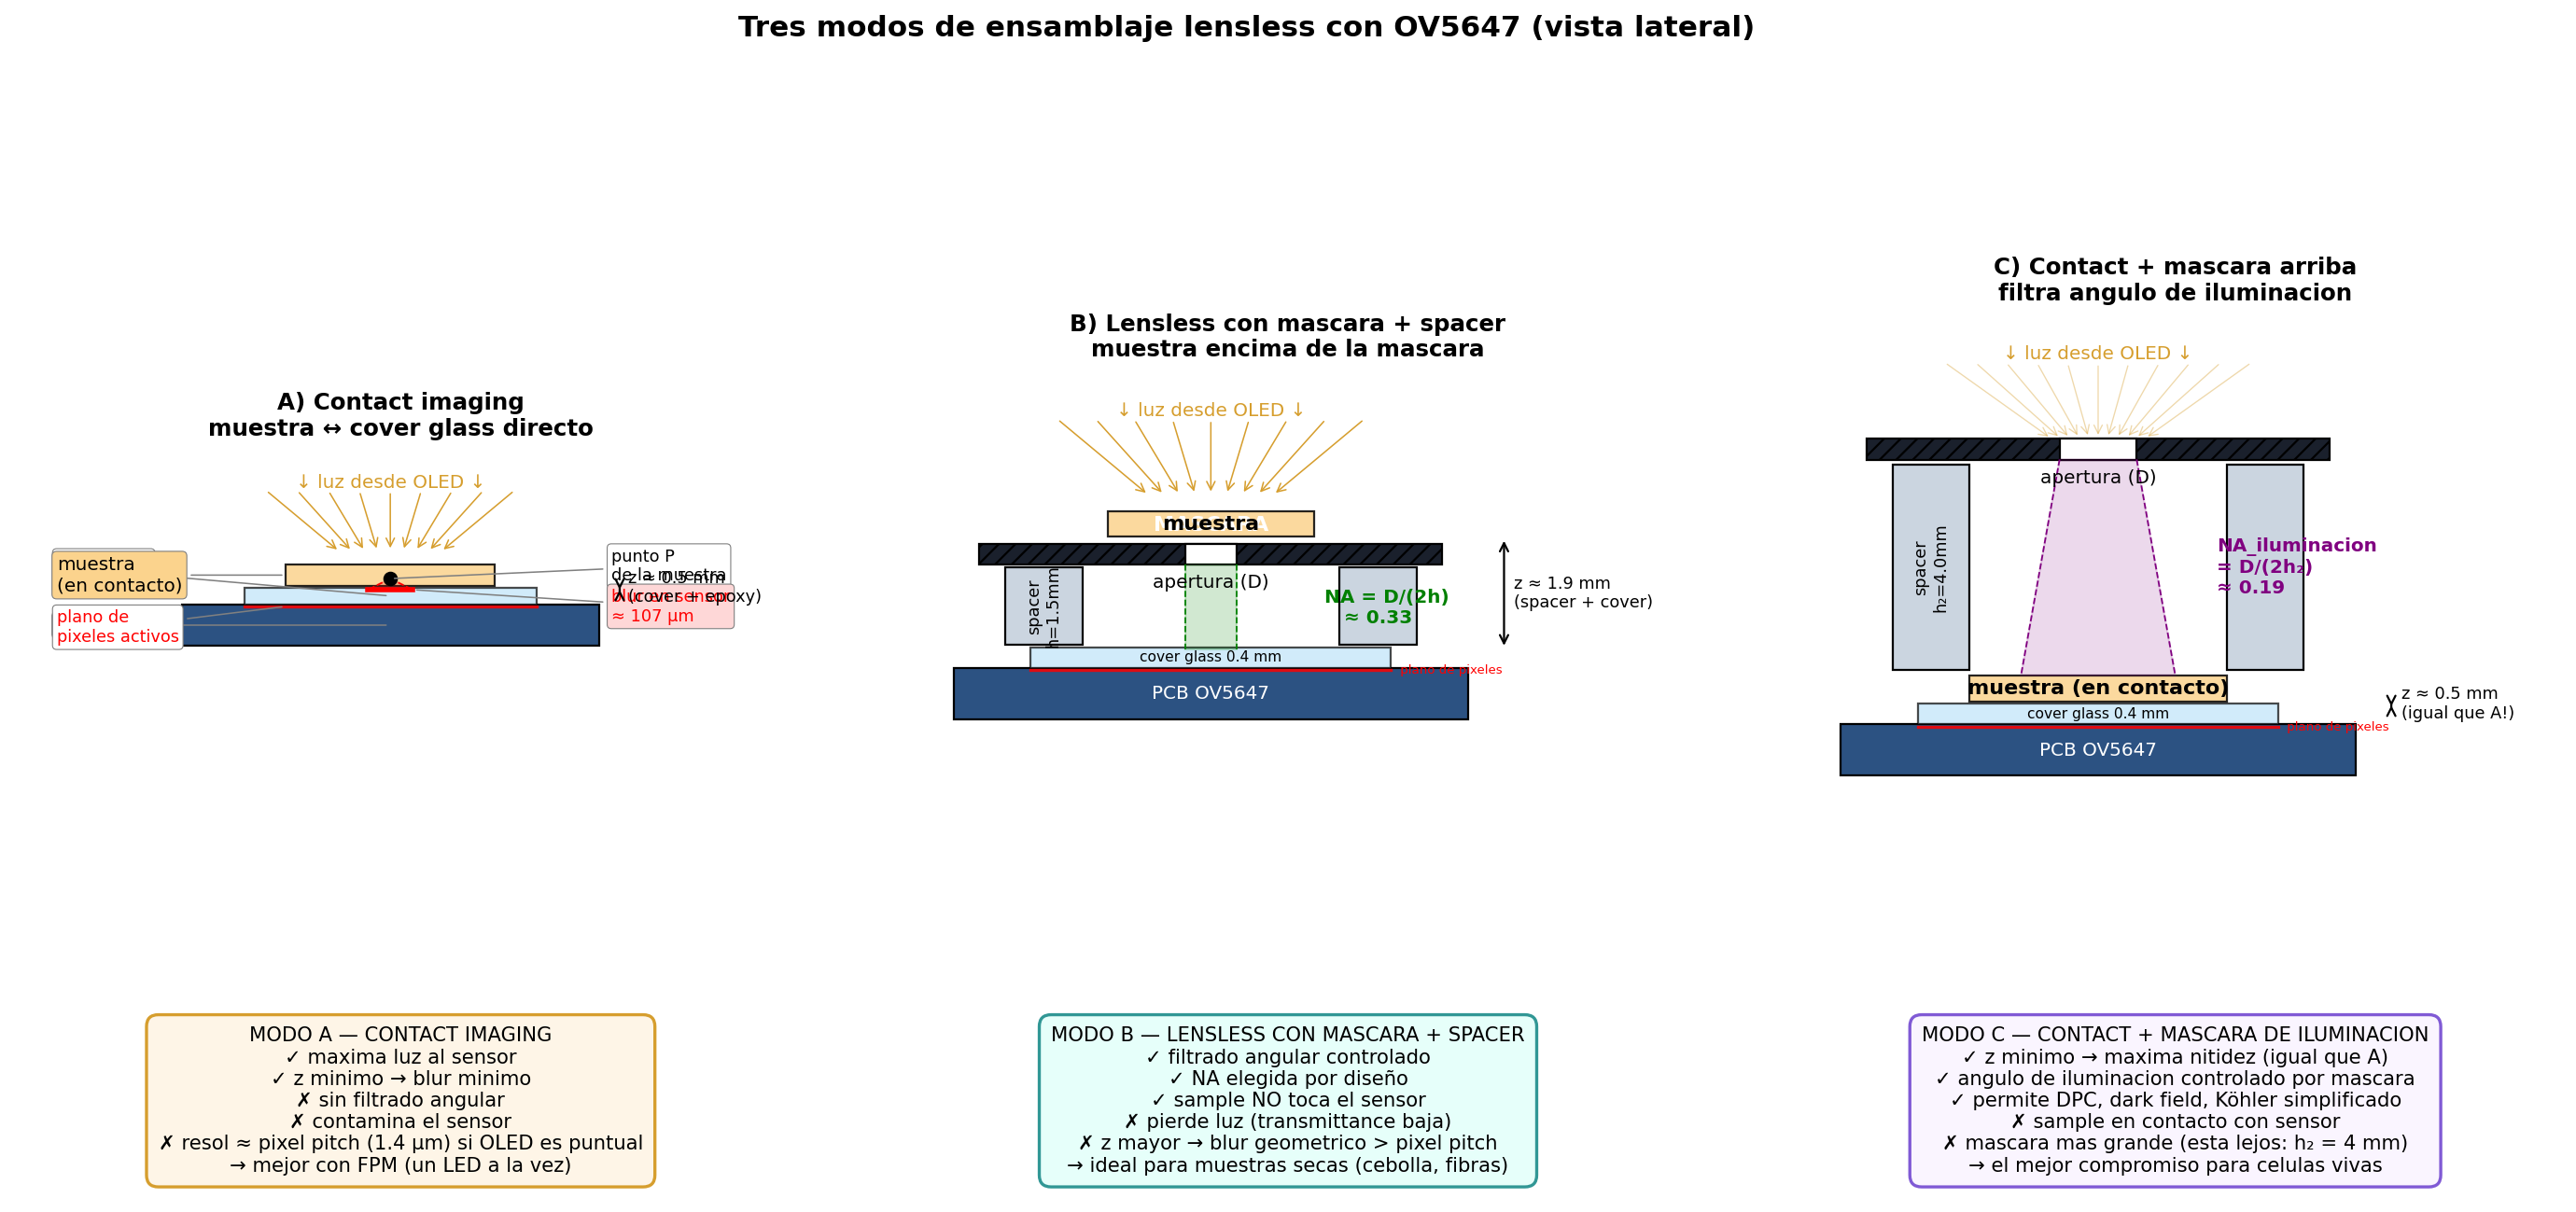
\includegraphics[width=\textwidth]{aperture_masks_assembly.png}
\caption{Comparacion esquematica de los tres modos de ensamblaje. (A) Contact
imaging directo sobre cover glass, sin mascara. (B) Configuracion lensless
clasica: muestra apoyada en la mascara, separada del sensor por un spacer.
(C) Configuracion hibrida: muestra en contacto con cover glass y mascara
en posicion superior para controlar el angulo de iluminacion.}
\label{fig:modos}
\end{figure}

\subsection{Modo A --- Contact imaging directo}

La muestra se apoya directamente sobre el cover glass del sensor. La
distancia efectiva muestra-pixel es $z \approx 0{,}5$ mm (cover glass
mas adhesivo). No hay mascara ni spacer.

\subsection{Modo B --- Lensless con mascara y spacer}

Se interpone la mascara entre la muestra y el cover glass, separada
por la altura del housing impreso. Para los housings actuales, la
distancia efectiva es $h = 5{,}0\;\mathrm{mm}$ (medida directa sobre
el modelo CAD final). La muestra se apoya sobre la mascara.

\subsection{Modo C --- Contact con mascara superior}

La muestra esta en contacto con el cover glass (igual que en A), pero
sobre ella se monta el housing y la mascara queda separada. La mascara
filtra angularmente la \emph{iluminacion} antes de que toque la muestra.

\section{Pipeline de procesamiento}

Las imagenes adquiridas son procesadas por el pipeline de IA del repositorio
\texttt{CubeSat-EdgeAI-Payload}, que ejecuta secuencialmente:

\begin{enumerate}[leftmargin=2.2em]
  \item Preprocesamiento (CLAHE, denoising no local).
  \item Segmentacion celular con StarDist (modelo \texttt{2D\_versatile\_he}).
  \item Calculo de metricas dimensionales (area, perimetro, circularidad,
        aspect ratio, solidez).
  \item Exportacion: \texttt{overlay.png}, \texttt{mask.png}, \texttt{data.csv},
        \texttt{summary.json}.
\end{enumerate}

% =====================================================================
\chapter{Diseño experimental}

\section{Matriz factorial}

Se utiliza un diseño factorial completo $3 \times 3$ con tres mascaras
y tres modos de ensamblaje. Cada combinacion se replica tres veces para
cuantificar la repetibilidad, totalizando $27$ capturas.

\begin{table}[h!]
\centering
\caption{Matriz experimental. Cada celda contiene la prediccion cualitativa
del comportamiento esperado.}
\renewcommand{\arraystretch}{1.4}
\begin{tabular}{p{2.5cm}p{3.5cm}p{3.5cm}p{4cm}}
\toprule
\textbf{Mascara $\backslash$ Modo} & \textbf{A) contact} & \textbf{B) lensless $+$ spacer} & \textbf{C) contact $+$ mascara arriba} \\
\midrule
\textbf{Slit} & shadow line scan con blur & line scan claro, perdida de luz & DPC con corte direccional \\
\textbf{Cuadrada} & FOV cuadrado borroso & FOV cuadrado nitido & iluminacion cuadrada controlada \\
\textbf{Pinhole} & FOV circular borroso & FOV circular nitido (referencia) & Köhler simplificado \\
\bottomrule
\end{tabular}
\label{tab:matriz}
\end{table}

\section{Variables controladas}

\begin{itemize}[leftmargin=2.2em]
  \item Misma muestra fisica en todas las capturas.
  \item Misma iluminacion: bright field uniforme del OLED.
  \item Mismo tiempo de exposicion (ajustado en una sola toma de
        referencia, fijado por las nueve condiciones).
  \item Misma temperatura ambiente y humedad.
  \item Mismo operador y momento del dia (factor a controlar para evitar
        sesgos de manipulacion).
\end{itemize}

\section{Metricas de evaluacion}

\begin{table}[h!]
\centering
\caption{Metricas cuantitativas evaluadas para cada captura.}
\renewcommand{\arraystretch}{1.4}
\small
\begin{tabular}{p{2.7cm}p{4.2cm}p{6.5cm}}
\toprule
\textbf{Metrica} & \textbf{Definicion} & \textbf{Procedimiento de medicion} \\
\midrule
Resolucion (FWHM) &
Ancho a media altura del perfil de un borde &
Ajuste de erf al perfil cruzado de una pared celular; FWHM derivada de la pendiente. \\
Contraste de Michelson &
$(I_{\max}{-}I_{\min}) / (I_{\max}{+}I_{\min})$ &
ROI de $50\times 50$ pixeles entre celula vs fondo. \\
SNR &
$\mu / \sigma$ en zona uniforme &
ROI de $100\times 100$ pixeles en region sin estructura. \\
FOV utilizable &
\% de pixels con varianza local arriba de un umbral &
Filtro Laplaciano + binarizacion + conteo. \\
Numero de celulas &
Salida del segmentador StarDist &
Ejecucion automatica del pipeline. \\
Brillo medio &
Valor de gris promedio &
Media global de la ROI muestra. \\
\bottomrule
\end{tabular}
\label{tab:metricas}
\end{table}

% =====================================================================
\chapter{Predicciones (con dimensiones reales)}

A continuacion se exponen las predicciones cuantitativas para cada mascara,
basadas en el marco teorico del Capitulo 2 y las dimensiones medidas en CAD.
Se utiliza el valor real $h = 5{,}0\;\mathrm{mm}$ medido sobre el housing
impreso (profundidad efectiva mascara-sensor).

\section{Pinhole circular Ø 3.000 mm}

\begin{figure}[h!]
\centering
\includegraphics[width=0.4\textwidth]{{Muesca Circular}.png}
\hspace{0.5cm}
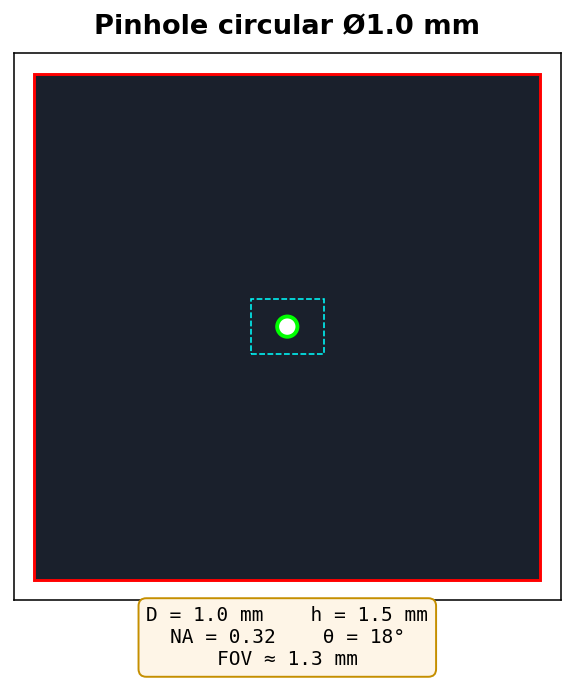
\includegraphics[width=0.4\textwidth]{pinhole_circular_d1.0_mm.png}
\caption{Pinhole circular Ø $3{,}000\;\mathrm{mm}$. Izquierda: CAD real.
Derecha: simulacion 2D de referencia (no a escala con la dimension real).}
\end{figure}

\begin{calculo}
Diametro $D = 3{,}000\;\mathrm{mm}$, $h = 5{,}0\;\mathrm{mm}$:
\[
\mathrm{NA} = \sin\!\left(\arctan\!\frac{D}{2h}\right) = \sin(\arctan(0{,}30)) = 0{,}287
\]
\[
d_{\min} = \frac{\lambda}{2\,\mathrm{NA}} = \frac{0{,}55}{2\cdot 0{,}287} \approx 0{,}96\;\mu\mathrm{m}
\]
\[
d_{\text{Airy}} = \frac{1{,}22\,\lambda}{2\,\mathrm{NA}} \approx 1{,}17\;\mu\mathrm{m}
\]
\textbf{Area} $= \pi (D/2)^2 = \pi \cdot 1{,}5^2 = 7{,}07\;\mathrm{mm}^2$.\\
Resolucion sub-micrometrica posible; el sensor (pixel $1{,}4\;\mu$m) es el limitante.
\end{calculo}

\begin{hipotesis}
\begin{itemize}[leftmargin=1.5em]
  \item FOV circular uniforme, simetrico bajo rotaciones.
  \item Resolucion isotropica $\sim 1\;\mu\mathrm{m}$.
  \item Anillos concentricos visibles cuando hay puntos brillantes saturados.
  \item PSF Airy con primer minimo en $r \approx 1\;\mu$m, comparable al pixel pitch.
  \item Mayor area de las tres geometrias $\Rightarrow$ mas luz $\Rightarrow$
        SNR alto. La hipotesis previa (pinhole con menor luz) cambia con la nueva
        geometria de Ø$\,3\;\mathrm{mm}$.
  \item Geometria de referencia para la calibracion del sistema y para
        el pipeline de segmentacion automatica (PSF mas predecible).
\end{itemize}
\end{hipotesis}

\section{Apertura cuadrada $3{,}054\times 3{,}054\;\mathrm{mm}$}

\begin{figure}[h!]
\centering
\includegraphics[width=0.4\textwidth]{{Muesca Cuadrada}.png}
\hspace{0.5cm}
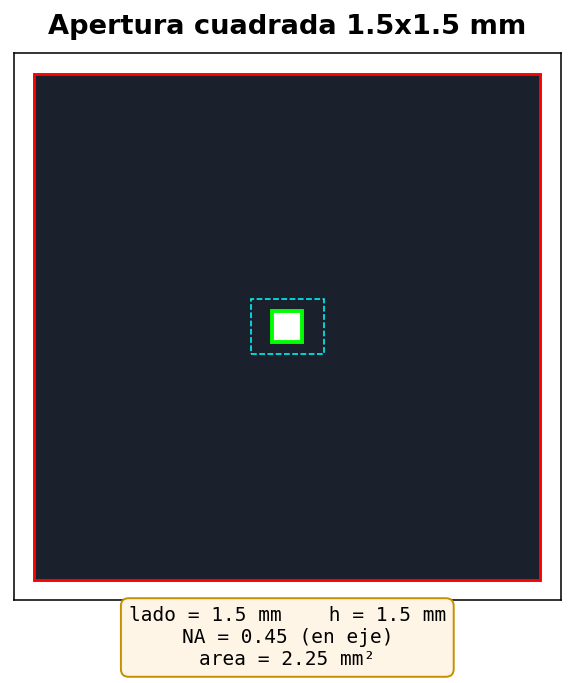
\includegraphics[width=0.4\textwidth]{apertura_cuadrada_1.5x1.5_mm.png}
\caption{Apertura cuadrada $3{,}054\;\mathrm{mm}$ de lado. Izquierda: CAD real.
Derecha: simulacion 2D de referencia.}
\end{figure}

\begin{calculo}
Lado $s = 3{,}054\;\mathrm{mm}$, $h = 5{,}0\;\mathrm{mm}$:
\[
\mathrm{NA}_{\text{eje}} = \sin(\arctan(s/2h)) = \sin(\arctan(0{,}305)) = 0{,}292
\]
\[
\mathrm{NA}_{\text{diag}} = \sin(\arctan(s\sqrt{2}/2h)) = \sin(\arctan(0{,}432)) = 0{,}396
\]
\[
d_{\min,\text{eje}} = \frac{0{,}55}{2\cdot 0{,}292} \approx 0{,}94\;\mu\mathrm{m}
\]
\textbf{Area} $= s^2 = 9{,}33\;\mathrm{mm}^2$ (la mas grande de las tres).
\end{calculo}

\begin{hipotesis}
\begin{itemize}[leftmargin=1.5em]
  \item FOV cuadrado bien definido con bordes rectos visibles.
  \item Resolucion uniforme en X e Y, anisotropica respecto a la diagonal.
  \item \textbf{Mayor flujo luminoso} de las tres mascaras (area $\times 1{,}32$ vs pinhole).
  \item Difraccion en esquinas: PSF separable $\mathrm{sinc}^2 \times \mathrm{sinc}^2$,
        con lobulos cruzados alineados a los ejes principales.
  \item Aplicacion preferida: imaging general con maxima area utilizable y
        maxima luz disponible.
\end{itemize}
\end{hipotesis}

\section{Rendija lineal $0{,}178\;\mathrm{mm} \times 5{,}606\;\mathrm{mm}$}

\begin{figure}[h!]
\centering
\includegraphics[width=0.4\textwidth]{{Muesca Rejilla}.png}
\hspace{0.5cm}
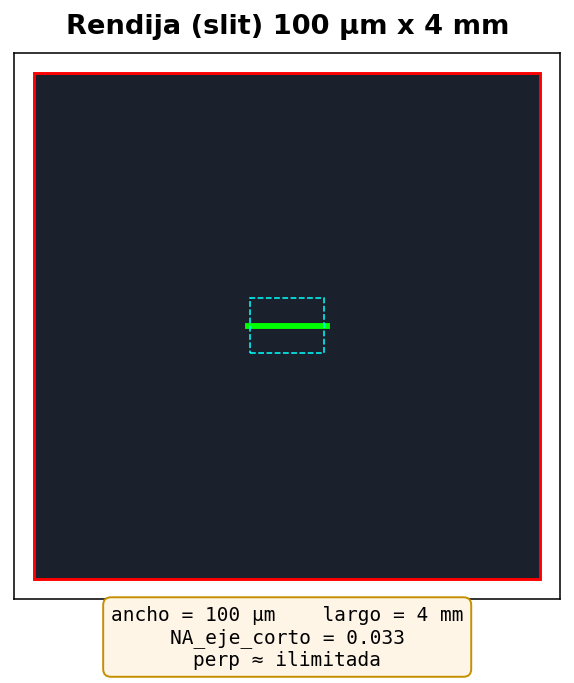
\includegraphics[width=0.4\textwidth]{rendija_(slit)_100_µm_x_4_mm.png}
\caption{Rendija lineal: ancho $0{,}178\;\mathrm{mm}$, largo $5{,}606\;\mathrm{mm}$,
con cinco ranuras replicadas en paralelo. Izquierda: CAD real. Derecha:
simulacion 2D de referencia.}
\end{figure}

\begin{calculo}
Eje corto ($w = 0{,}178\;\mathrm{mm}$, $h = 5{,}0\;\mathrm{mm}$):
\[
\mathrm{NA}_{\text{corto}} = \frac{w}{2h} = 0{,}0178 \quad\Rightarrow\quad
d_{\min} \approx \frac{\lambda}{2\,\mathrm{NA}} \approx 15{,}4\;\mu\mathrm{m}
\]
Eje largo ($L = 5{,}606\;\mathrm{mm}$):
\[
\mathrm{NA}_{\text{largo}} = \sin(\arctan(L/2h)) = \sin(\arctan(0{,}561)) = 0{,}489
\]
\textbf{Area de una ranura} $= 0{,}178 \times 5{,}606 = 0{,}998\;\mathrm{mm}^2$
$\;\to\;$ con cinco ranuras: $\approx 5{,}0\;\mathrm{mm}^2$.
\end{calculo}

\begin{hipotesis}
\begin{itemize}[leftmargin=1.5em]
  \item Resolucion baja ($\sim 15\;\mu$m) en el eje perpendicular a la rendija
        --- significativamente peor que las otras dos.
  \item Resolucion alta ($\sim 1\;\mu$m) en el eje paralelo.
  \item Imagen de tipo \emph{multi-line scan} (cinco bandas de luz paralelas).
  \item SNR moderado --- comparable a la cuadrada cuando se suman las cinco ranuras.
  \item Aplicacion preferida: perfilometria y line-scanning con rotacion mecanica
        de la muestra; tambien util para experimentos de difraccion controlada.
  \item \textbf{Cambio respecto al diseño anterior:} el ancho de $178\;\mu$m
        (vs $100\;\mu$m supuesto) reduce la NA del eje corto en $44\%$,
        empeorando la resolucion teorica.
\end{itemize}
\end{hipotesis}

\section{Predicciones agregadas}

\begin{table}[h!]
\centering
\caption{Sintesis cualitativa de las predicciones, asumiendo $h = 5{,}0\;\mathrm{mm}$.
$\bullet\bullet\bullet$ indica rendimiento esperado superior; $\bullet$ marginal.}
\renewcommand{\arraystretch}{1.4}
\begin{tabular}{p{4.5cm}ccc}
\toprule
 & \textbf{Slit} & \textbf{Cuadrada} & \textbf{Pinhole} \\
\midrule
Resolucion eje fino             & $\bullet$               & $\bullet\bullet\bullet$ & $\bullet\bullet\bullet$ \\
Resolucion uniforme             & ---                     & $\bullet\bullet\bullet$ & $\bullet\bullet\bullet$ \\
Flujo luminoso / SNR            & $\bullet\bullet$        & $\bullet\bullet\bullet$ & $\bullet\bullet$  \\
Campo de vision utilizable      & $\bullet$ (linea)       & $\bullet\bullet\bullet$ & $\bullet\bullet$  \\
Predictibilidad de la PSF       & $\bullet\bullet$        & $\bullet\bullet$        & $\bullet\bullet\bullet$ \\
Aplicacion preferida            & line-scan, perfilometria & lensless general & calibracion, referencia \\
\bottomrule
\end{tabular}
\label{tab:predicciones}
\end{table}

\paragraph{Cambio de jerarquia respecto a la version anterior.}
La duplicacion del diametro del pinhole ($1{,}0 \to 3{,}0\;\mathrm{mm}$) y de
la cuadrada ($1{,}5 \to 3{,}054\;\mathrm{mm}$) iguala la NA y la resolucion
entre ambas. La cuadrada ahora es la mascara con \emph{mas} flujo luminoso
(area $9{,}33\;\mathrm{mm}^2$ vs $7{,}07\;\mathrm{mm}^2$ del pinhole). El
slit, en cambio, mantiene su nicho como detector anisotropico.

% =====================================================================
\chapter{Procedimiento experimental}

\section{Etapa 1 --- Calibracion previa}

\begin{enumerate}[leftmargin=2.2em]
  \item Verificar dimensiones reales de cada mascara fabricada con calibre
        digital o microscopio de inspeccion. Comparar contra los valores CAD:
        Ø$\,3{,}000\;\mathrm{mm}$ pinhole, $3{,}054\;\mathrm{mm}$ cuadrada,
        $0{,}178 \times 5{,}606\;\mathrm{mm}$ rejilla. Registrar discrepancias en
        \texttt{exp\_<fecha>/calibration.json}.
  \item Capturar imagen de la regleta de $1$ mm en cada modo (A, B, C)
        para determinar el factor $\mu$m/pixel real, no asumir el valor
        por defecto de $2{,}66$. Registrar en el log experimental.
  \item Verificar la uniformidad espacial de la iluminacion del OLED
        capturando una imagen \emph{flat-field} sin muestra; esta servira
        para correccion post-hoc.
  \item Medir la altura efectiva del housing $h$ con calibre. Usar este
        valor real en lugar del $h = 5{,}0\;\mathrm{mm}$ asumido en los
        calculos teoricos.
\end{enumerate}

\section{Etapa 2 --- Preparacion}

\begin{enumerate}[leftmargin=2.2em]
  \item Limpiar el cover glass del sensor con isopropilico al $99\%$ y
        un paño de microfibra libre de pelusas.
  \item Preparar la muestra de epidermis de cebolla, montada entre
        coverslips de vidrio. Almacenar entre capturas en camara humeda.
  \item Verificar el tiempo de exposicion del sensor con la mascara mas
        restrictiva (slit, $\sim 1\;\mathrm{mm}^2$ de area por ranura) para
        no saturar en la mas abierta (cuadrada, $9{,}33\;\mathrm{mm}^2$);
        fijarlo para todas las nueve condiciones.
\end{enumerate}

\section{Etapa 3 --- Adquisicion}

Para cada combinacion de las nueve condiciones experimentales:

\begin{enumerate}[leftmargin=2.2em]
  \item Montar la mascara correspondiente con su housing.
  \item Verificar la distancia $h$ con calibre.
  \item Disparar tres capturas consecutivas mediante:
\begin{verbatim}
python -m cubesat.daemon --capture --tag exp_<mask>_<mode>_<rep>
\end{verbatim}
  \item Verificar que el histograma de cada captura este centrado, sin
        clipping en los extremos.
  \item Registrar tiempo de exposicion final, hora de la captura y
        condiciones ambientales en el log.
\end{enumerate}

\section{Etapa 4 --- Procesamiento}

\begin{enumerate}[leftmargin=2.2em]
  \item Ejecutar el pipeline completo:
\begin{verbatim}
python -m pipeline.controller run --input exp_<fecha>/
\end{verbatim}
  \item Para cada captura, el pipeline genera \texttt{overlay.png},
        \texttt{mask.png}, \texttt{data.csv} y \texttt{summary.json}.
  \item Consolidar todos los \texttt{summary.json} en una tabla pivot
        agrupada por mascara y modo.
\end{enumerate}

\section{Etapa 5 --- Analisis}

\begin{enumerate}[leftmargin=2.2em]
  \item Por cada metrica de la Tabla \ref{tab:metricas}, generar un boxplot
        con $9$ celdas (3 mascaras $\times$ 3 modos), $3$ replicas por celda.
  \item Realizar test estadisticos (ANOVA de dos vias, $\alpha = 0{,}05$)
        para evaluar significancia de los efectos principales y la interaccion.
  \item Confirmar o refutar las predicciones de la Tabla \ref{tab:predicciones}.
  \item Identificar resultados inesperados; investigar causa fisica posible.
  \item Documentar conclusiones en \texttt{exp\_<fecha>/RESULTS.md} y
        publicar el conjunto de datos crudos en GitHub bajo
        \texttt{experiments/<fecha>\_mascaras/}.
\end{enumerate}

% =====================================================================
\chapter{Limitaciones y trabajo futuro}

\section{Limitaciones del experimento propuesto}

\begin{limitacion}
\begin{itemize}[leftmargin=1.5em]
  \item \textbf{Tolerancias de fabricacion.} Las dimensiones medidas en CAD
        (especialmente el ancho de rendija $w = 0{,}178\;\mathrm{mm}$) deben
        verificarse en la pieza fabricada. Una desviacion de $\pm 50\;\mu$m
        modifica la NA en un $\pm 28\%$ y altera todas las predicciones
        cuantitativas.
  \item \textbf{Distancia $h$ del housing.} El valor $h = 5{,}0\;\mathrm{mm}$
        proviene del modelo CAD; la pieza fabricada puede tener desviaciones
        de impresion 3D del orden de $\pm 0{,}1\;\mathrm{mm}$, lo que cambia
        la NA en $\pm 2\%$. Verificar con calibre.
  \item \textbf{Alineacion mecanica.} Un descentrado de $0{,}5$ mm entre
        la mascara y el sensor produce sombras en la imagen. Se mitiga con
        anclaje preciso por orejas con tornillos M2 y verificacion visual
        de la simetria del FOV.
  \item \textbf{Iluminacion no uniforme.} El OLED puede presentar gradientes
        radiales o de pixel a pixel. Se mitiga con la captura de
        \emph{flat-field} y normalizacion post-hoc.
  \item \textbf{Reflexiones internas.} Si la cara superior del housing no
        es opaca y mate, aparecen reflejos cruzados. Se mitiga con PLA
        negro mate o anodizado.
  \item \textbf{Contaminacion.} Una particula de polvo en la mascara
        produce un punto fijo en todas las capturas. Se mitiga con
        limpieza con aire comprimido y verificacion visual previa.
\end{itemize}
\end{limitacion}

\section{Trabajo futuro}

Una vez completado el experimento descrito, las siguientes lineas de
investigacion son recomendables:

\begin{enumerate}[leftmargin=2.2em]
  \item \textbf{FPM con iluminacion puntual.} Repetir las nueve condiciones
        usando un solo LED encendido a la vez, en una grilla $5 \times 5$ del
        OLED. Esto permite reconstruccion ptychografica con resolucion
        sintetizada superior al limite de Abbe nominal.
  \item \textbf{Mascara honeycomb.} Evaluar un arreglo de pinholes paralelos
        como cuarta geometria.
  \item \textbf{Differential Phase Contrast (DPC).} Implementar la mascara
        del modo C en cuatro orientaciones (left/right/top/bottom) para
        reconstruir el mapa de fase de objetos transparentes.
  \item \textbf{Caracterizacion de profundidad de campo.} Medir el rango
        axial de buena nitidez para cada mascara variando la distancia
        muestra-sensor.
  \item \textbf{Integracion al payload final.} Seleccionar la mascara
        ganadora y disenar su housing definitivo para integrarla al
        modelo de vuelo del CubeSat.
\end{enumerate}

% =====================================================================
\chapter{Conclusion}

Este informe presenta una propuesta experimental sistematica para
caracterizar tres geometrias de apertura optica en el contexto de un
payload de microscopia lensless integrado a un CubeSat. Las dimensiones
finales de las mascaras provienen de medicion directa sobre el modelo CAD
en Autodesk Inventor y son: pinhole circular $\varnothing\,3{,}000\;\mathrm{mm}$,
apertura cuadrada $3{,}054 \times 3{,}054\;\mathrm{mm}$ y rendija lineal
$0{,}178 \times 5{,}606\;\mathrm{mm}$.

La metodologia propuesta es factorial completa, replicada y cuantitativa,
con predicciones especificas derivadas del marco teorico de optica de
Fourier. Las metricas seleccionadas (FWHM, contraste de Michelson, SNR,
fraccion de FOV utilizable, numero de celulas detectadas y brillo medio)
permiten un analisis multidimensional del rendimiento de cada configuracion.

Bajo las dimensiones reales del CAD con $h = 5{,}0\;\mathrm{mm}$ (profundidad
medida del housing impreso):

\begin{itemize}[leftmargin=2em]
  \item El \textbf{pinhole circular} y la \textbf{apertura cuadrada}
        tienen NA practicamente identica ($0{,}287$ vs $0{,}292$) y
        resolucion teorica $\sim 1\;\mu\mathrm{m}$. La diferencia clave
        es geometrica: simetria circular vs cuadrada de la PSF.
  \item La \textbf{cuadrada} ofrece $32\%$ mas area que el pinhole
        $\Rightarrow$ mas luz disponible.
  \item El \textbf{slit} tiene NA un orden de magnitud menor en su eje fino
        (resolucion $\sim 15\;\mu\mathrm{m}$) y se reserva para perfilometria
        anisotropica.
\end{itemize}

La validacion experimental de estas predicciones constituye un paso
necesario para la seleccion definitiva de la mascara que se integrara al
modelo de vuelo del payload.

% =====================================================================
\chapter*{Bibliografia}
\addcontentsline{toc}{chapter}{Bibliografia}

{\small
\noindent
\begin{enumerate}[leftmargin=2em]
\item Goodman JW. \emph{Introduction to Fourier Optics}. 4ed. W.H. Freeman, 2017.
\item Born M, Wolf E. \emph{Principles of Optics}. 7ed. Cambridge University Press, 1999.
\item Mertz J. \emph{Introduction to Optical Microscopy}. 2ed. Cambridge University Press, 2019.
\item Zheng G, Horstmeyer R, Yang C. Wide-field, high-resolution Fourier
ptychographic microscopy. \emph{Nature Photonics} 7:739-745, 2013.
\item Greenbaum A, et al. Imaging without lenses: achievements and remaining challenges of wide-field on-chip microscopy. \emph{Nature Methods} 9:889-895, 2012.
\item Tian L, Waller L. Quantitative differential phase contrast imaging in an LED array microscope. \emph{Optics Express} 23:11394-11403, 2015.
\item Schmidt U, Weigert M, Broaddus C, Myers G. Cell Detection with Star-Convex Polygons. \emph{MICCAI}, 2018.
\item OmniVision Technologies. \emph{OV5647 Color CMOS QSXGA (5 Megapixel) Image Sensor with OmniBSI Technology}. Datasheet, 2009.
\end{enumerate}
}

\end{document}
